\documentclass[11pt,a4paper]{article}

\usepackage[utf8]{inputenc}
\usepackage[spanish]{babel}
\usepackage{amsmath}
\usepackage{amsfonts}
\usepackage{amssymb}
\usepackage{makeidx}
\usepackage{graphicx}
\usepackage{lmodern}
\usepackage{kpfonts}
\usepackage{wrapfig}
\usepackage{caption}
\usepackage{subcaption}
\usepackage{booktabs}
\usepackage[nottoc,numbib]{tocbibind} %agrega la bibliografia al índice.
\usepackage[font={small,it}]{caption}
%\usepackage{fourier}
\usepackage[left=2cm,right=2cm,top=2cm,bottom=2cm,headheight=13.6pt]{geometry}
\usepackage{fancyhdr}
\pagestyle{fancy}


%Para los gráficos en general, con las tablas...¡Ja!, arreglate.
%\begin{figure}[h!]
%\centering
%\includegraphics[width=0.7\textwidth]{} %nombre de la imagen, incluirla en el mismo directorio que este archivo.
%\caption*{} %rótulo, el asterico elimina la numeración automática. 
%\label{fig:} % para luego referirse con \ref{fig:}
%\end{figure}


\begin{document}


%%%%%%%%%%%%%%%%%%%%%%%%%%%%%%%%%%%%%%%%%%%%%%%%%%%%%%%%%%%%%%%%%%%%%%%%%%%%%%%%%%%%%%%%%%%%%%%%%%%%%%%%%%%%%%%%%%%%%%%%%%%%%%%%%
% 	TÍTULO
%%%%%%%%%%%%%%%%%%%%%%%%%%%%%%%%%%%%%%%%%%%%%%%%%%%%%%%%%%%%%%%%%%%%%%%%%%%%%%%%%%%%%%%%%%%%%%%%%%%%%%%%%%%%%%%%%%%%%%%%%%%%%%%%%

%%%%%%%%%%%%%%%%%%%%%%%%%%%%%%%%%%%%%%%%%
% University Assignment Title Page 
% LaTeX Template
% Version 1.0 (27/12/12)
%
% This template has been downloaded from:
% http://www.LaTeXTemplates.com
%
% Original author:
% WikiBooks (http://en.wikibooks.org/wiki/LaTeX/Title_Creation)
%
% License:
% CC BY-NC-SA 3.0 (http://creativecommons.org/licenses/by-nc-sa/3.0/)
% 
% Instructions for using this template:
% This title page is capable of being compiled as is. This is not useful for 
% including it in another document. To do this, you have two options: 
%
% 1) Copy/paste everything between \begin{document} and \end{document} 
% starting at \begin{titlepage} and paste this into another LaTeX file where you 
% want your title page.
% OR
% 2) Remove everything outside the \begin{titlepage} and \end{titlepage} and 
% move this file to the same directory as the LaTeX file you wish to add it to. 
% Then add \input{./title_page_1.tex} to your LaTeX file where you want your
% title page.
%
%%%%%%%%%%%%%%%%%%%%%%%%%%%%%%%%%%%%%%%%%

%----------------------------------------------------------------------------------------
%	PACKAGES AND OTHER DOCUMENT CONFIGURATIONS
%----------------------------------------------------------------------------------------

%\documentclass[12pt]{article}
%\usepackage[utf8]{inputenc}
%\usepackage[spanish]{babel}
%\begin{document}

\begin{titlepage}

\newcommand{\HRule}{\rule{\linewidth}{0.5mm}} % Defines a new command for the horizontal lines, change thickness here

\center % Center everything on the page
 
%----------------------------------------------------------------------------------------
%	HEADING SECTIONS
%----------------------------------------------------------------------------------------

\textsc{\Huge Universidad de Buenos Aires}\\[0.5cm]
\textsc{\LARGE Facultad de Ciencias Exactas y Naturales}\\[0.5cm] % Name of your university/college
\textsc{\Large Departamento de Física}\\[0.25cm] % Major heading such as course name

\begin{figure}[h]
  \centering
  
\includegraphics[scale=0.15]{Logo_DF}
  \\[0.5cm]
\end{figure}

\textsc{\large Laboratorio 3}\\[0.25cm] % Minor heading such as course title

%----------------------------------------------------------------------------------------
%	TITLE SECTION
%----------------------------------------------------------------------------------------

\HRule \\[0.4cm]
{ \huge \bfseries Transitorio y tiempo caracteristico de circuitos}\\[0.2cm] % Title of your document
\HRule \\[1cm]
 
%----------------------------------------------------------------------------------------
%	AUTHOR SECTION
%----------------------------------------------------------------------------------------

\begin{minipage}{0.4\textwidth}
\begin{center} \large
\emph{Autores:}\\
\textsc{Andreu}, Gonzalo\\ % Your name
\textsc{Malpartida}, Bryan\\ % Your name
\textsc{Pugliese}, Facundo\\ % Your name


\end{center}
\end{minipage}
~ \\[1.25cm]
%\begin{minipage}{0.4\textwidth}
%\begin{flushright} \large
%\emph{Supervisor:} \\
%Dr. James \textsc{Smith} % Supervisor's Name
%\end{flushright}
%\end{minipage}\\[4cm]

% If you don't want a supervisor, uncomment the two lines below and remove the section above
%\Large \emph{Author:}\\
%John \textsc{Smith}\\[3cm] % Your name

%----------------------------------------------------------------------------------------
%	DATE SECTION
%----------------------------------------------------------------------------------------

%\vspace{\fill}


{\large 17 de Febrero de 2016}\\[1.75cm] % Date, change the \today to a set date if you want to be precise

%----------------------------------------------------------------------------------------
%	SUMMARY SECTION: No más de 15 renglones, no te zarpes
%----------------------------------------------------------------------------------------

\begin{center}
\large{\textbf{Resumen}}

\small{El objetivo del siguiente trabajo fue caracterizar circuitos RC, RL y RCL. 

Para los dos primeros casos, los circuitos RC y RL, se buscó determinar el tiempos característico de cada uno variando los parámetros de cada sistema. Ademas de poder observar los fenómenos particulares en estos sistemas, como la carga y descarga del capacitor y la disminución de la corriente debido a la inductancia, utilizando una fuente de alimentación que emitía señales cuadradas y osciloscopio como instrumento de medición.

Por otro lado, el estudio del circuito RCL se centró en la observación de los comportamientos que tiene el mismo para distintos parámetros del sistema. Para ellos se obtenían teóricamente los valores necesarios de cada parámetro para luego $settear$ los elementos del circuito y comprobar que la evolución del sistema cumpliese el modelo teórico. Dichas observaciones se obtuvieron nuevamente utilizando una fuente de señal cuadrada y un osciloscopio.

Finalmente, el método resulto eficiente a la hora de comprobar las ecuaciones referidas al circuito RC y, en menor medida, al circuito RL. En el caso del circuito RCL, pudieron analizarse los casos extremos de comportamiento, pero no el comportamiento borde debido a lo fino del mismo.} % ACA VA EL RESUMEN

\end{center}


%----------------------------------------------------------------------------------------
%	LOGO SECTION
%----------------------------------------------------------------------------------------

%\includegraphics{Logo}\\[1cm] % Include a department/university logo - this will require the graphicx package
 
%----------------------------------------------------------------------------------------

\vfill % Fill the rest of the page with whitespace

\end{titlepage}
%\end{document} %incluir en el mismo directorio que este archivo. Equivalente a un copiar-pegar, nada de andar diciendo \begin{document} en la portada. Dejar el nombre de Caratula a la caratula.

%%%%%%%%%%%%%%%%%%%%%%%%%%%%%%%%%%%%%%%%%%%%%%%%%%%%%%%%%%%%%%%%%%%%%%%%%%%%%%%%%%%%%%%%%%%%%%%%%%%%%%%%%%%%%%%%%%%%%%%%%%%%%%%%%
% 	ENCABEZADO Y PIE DE PÁGINA.
%%%%%%%%%%%%%%%%%%%%%%%%%%%%%%%%%%%%%%%%%%%%%%%%%%%%%%%%%%%%%%%%%%%%%%%%%%%%%%%%%%%%%%%%%%%%%%%%%%%%%%%%%%%%%%%%%%%%%%%%%%%%%%%%%

\lhead{}
\chead{}
\rhead{Laboratorio 3}
\lfoot{}
\cfoot{}
\rfoot{\thepage}
\renewcommand{\headrulewidth}{1pt}
\renewcommand{\footrulewidth}{1pt}


%%%%%%%%%%%%%%%%%%%%%%%%%%%%%%%%%%%%%%%%%%%%%%%%%%%%%%%%%%%%%%%%%%%%%%%%%%%%%%%%%%%%%%%%%%%%%%%%%%%%%%%%%%%%%%%%%%%%%%%%%%%%%%%
% Página en blanco. Cita, agradecimiento, dedicación, lo que sea pero que sea algo.
%%%%%%%%%%%%%%%%%%%%%%%%%%%%%%%%%%%%%%%%%%%%%%%%%%%%%%%%%%%%%%%%%%%%%%%%%%%%%%%%%%%%%%%%%%%%%%%%%%%%%%%%%%%%%%%%%%%%%%%%%%%%%%%


%%%%%%%%%%%%%%%%%%%%%%%%%%%%%%%%%%%%%%%%%%%%%%%%%%%%%%%%%%%%%%%%%%%%%%%%%%%%%%%%%%%%%%%%%%%%%%%%%%%%%%%%%%%%%%%%%%%%%%%%%%%%%%%%%
% 	ÍNDICE
%%%%%%%%%%%%%%%%%%%%%%%%%%%%%%%%%%%%%%%%%%%%%%%%%%%%%%%%%%%%%%%%%%%%%%%%%%%%%%%%%%%%%%%%%%%%%%%%%%%%%%%%%%%%%%%%%%%%%%%%%%%%%%%%%

%\tableofcontents %compilar dos o tres veces para verlo bien. ¡Todo un índice en unas cuantas letras!
%\newpage

%%%%%%%%%%%%%%%%%%%%%%%%%%%%%%%%%%%%%%%%%%%%%%%%%%%%%%%%%%%%%%%%%%%%%%%%%%%%%%%%%%%%%%%%%%%%%%%%%%%%%%%%%%%%%%%%%%%%%%%%%%%%%%%
% 1. RESUMEN
%%%%%%%%%%%%%%%%%%%%%%%%%%%%%%%%%%%%%%%%%%%%%%%%%%%%%%%%%%%%%%%%%%%%%%%%%%%%%%%%%%%%%%%%%%%%%%%%%%%%%%%%%%%%%%%%%%%%%%%%%%%%%%%

\section{Resumen}
\label{sec:resumen}



%%%%%%%%%%%%%%%%%%%%%%%%%%%%%%%%%%%%%%%%%%%%%%%%%%%%%%%%%%%%%%%%%%%%%%%%%%%%%%%%%%%%%%%%%%%%%%%%%%%%%%%%%%%%%%%%%%%%%%%%%%%%%%%
% 2. INTRODUCCIÓN: ecuaciones aquí, luego se las cita.
%%%%%%%%%%%%%%%%%%%%%%%%%%%%%%%%%%%%%%%%%%%%%%%%%%%%%%%%%%%%%%%%%%%%%%%%%%%%%%%%%%%%%%%%%%%%%%%%%%%%%%%%%%%%%%%%%%%%%%%%%%%%%%%

\section{Introducción}\label{sec:intro}

El siguiente informe detalla los experimentos llevados a cabo para comprobar empíricamente dos de las herramientas fundamentales a la hora de resolver un circuito eléctrico: la ley de Ohm y el teorema de Thevenin. Ademas, comprobar empíricamente la ley de Joule, que determina la potencia disipada por una resistencia, y la eficacia de la misma.

La ley de Ohm dice que si una fuente $\varepsilon$ y una resistencia $R$ están conectados en serie, la diferencia de potencial entre las terminales $A$ y $B$ (en los extremos de este circuito respectivamente) es $V_{AB} = \varepsilon –iR$, donde $i$ es la corriente eléctrica generada por la fuente que pasa por la resistencia. En particular, si el circuito es cerrado se tiene $V_{AB}=0$ obteniendo entonces:

\begin{equation}\label{Ohm}
\ i= \frac{\varepsilon}{R}
\end{equation}

Por otro lado, el teorema de Thevenin enuncia que si se desea conocer el comportamiento de un circuito en una sola rama el resto del circuito puede reemplazarse por una rama que consiste de una resistencia equivalente $R_{th}$ y una fuente equivalente $\varepsilon_{th}$.

La resistencia $R_{th}$ se calcula cortando el circuito y resolviendo el sistema de resistencias que se obtiene. Mientras que la fuente equivalente $\varepsilon_{th}$ se obtiene calculando la diferencia de potencial entre $A$ y $B$ a circuito abierto utilizando las corrientes previamente calculadas mediante, por ejemplo, el método de ramas.

Para el sistema utilizado (detallado mas adelante) se tiene:

\begin{equation}\label{Rth}
\ R_{th}= \frac{rR}{2r+R}
\end{equation}

\begin{equation}\label{Eth}
\ \varepsilon_{th}= \frac{2\varepsilon r}{2r+R}
\end{equation}

Por ultimo, para poder calcular la potencia disipada por una resistencia $R$, la ley de Joule determina la siguiente ecuación:

\begin{equation}\label{Joule}
\ P = i^2 R
\end{equation}

Donde la $i$ es la corriente que pasa por la resistencia. 

De esta forma, si se coloca una resistencia de carga $R_{v}$ que pueda variar en paralelo con una resistencia de un circuito, y calculando su respectivo equivalente de Thevenin, se puede obtener la potencia disipada por $R_{v}$ como:

\begin{equation}\label{Pot}
\ P_{R_{v}}=\frac{\varepsilon_{th}^2 R_{v}}{(R_{v}+R_{th})^2}
\end{equation}

Una curva acampanada cuyo máximo debería encontrarse en $R_{max} = R_{th}$.

Sin embargo, maxima disipación no implica máxima eficiencia. Por lo tanto, se define la eficacia como el cociente entre la potencia disipada por una resistencia $R$ y la potencia entregada por una fuente $\varepsilon$:

\begin{equation}\label{eficacia}
\ E=\frac{P_{R}}{P_{\varepsilon}}
\end{equation}

Por lo tanto, si se quiere conocer la eficacia de una resistencia $R$ se puede calcular su equivalente de Thevenin para obtener la relación:

\begin{equation}\label{efi}
\ E= \frac{\varepsilon_{th}}{\varepsilon}\frac{1}{1+\frac{R_{th}}{R}}
\end{equation}

%%%%%%%%%%%%%%%%%%%%%%%%%%%%%%%%%%%%%%%%%%%%%%%%%%%%%%%%%%%%%%%%%%%%%%%%%%%%%%%%%%%%%%%%%%%%%%%%%%%%%%%%%%%%%%%%%%%%%%%%%%%%%%%
% 3. DISPOSITIVO EXPERIMENTAL: armado del modelo, como se midio, consideraciones a la hora de medir.
%%%%%%%%%%%%%%%%%%%%%%%%%%%%%%%%%%%%%%%%%%%%%%%%%%%%%%%%%%%%%%%%%%%%%%%%%%%%%%%%%%%%%%%%%%%%%%%%%%%%%%%%%%%%%%%%%%%%%%%%%%%%%%%

\section{Desarrollo experimental}

\subsection{Ley de Ohm}

Como se ha dicho, una de las leyes basicas de los circuitos en general es la Ley de Ohm \textbf{\eqref{Ohm}}. Es por esto que la primer parte del trabajo se desarrolló en torno a su comprobación empírica para circuitos de corriente continua. El montaje del sistema fue simple, consistiendo en una Fuente de Alimentación Programable de 3 canales, un multimetro digital y una resistencia variable por decadas. La Fuente de Alimentación actuó como una fuente de voltaje constante, que se conectó en serie con el multimetro y la resistencia variable. Esto permitió generar un circuito de una única malla que consiste en una resistencia y una fuente de voltaje constante (Ver \textbf{Fig \ref{fig:circ_simp}}).


\begin{figure}[h]
  \centering
  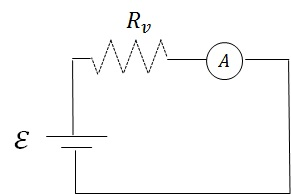
\includegraphics[scale= 0.6]{Circuito_simple}
  \caption{Circuito de malla única utilizado para la experiencia}
  \label{fig:circ_simp}
\end{figure}

La resistencia del multimetro utilizado en su función de amperímetro era $R_{A} = (11,8 \pm 0,4) \Omega$, la cual debió sumarse a la resistencia variable $R_v$ (pues están en serie) a la hora de calcular la resistencia total del circuito. La resistencia interna de la Fuente se asumió despreciable. Para empezar, se fijó la resistencia variable $R_v = (500 \pm 5)\Omega$ y se fue variando el voltaje de entrada $\varepsilon$, registrándose la corriente $I$ resultante para cada valor de $\varepsilon$. Posteriormente, utilizando el mismo circuito se planteó analizar la relación entre $I$ y $R$ fijando el voltaje de la fuente a $\varepsilon = (15,0 \pm 0,1)V$ y variando la resistencia total $R = R_v + R_A$ a través de $R_v$. 


\subsection{Equivalente de Thevenin y Ley de Joule}

Terminado lo anterior, se propuso montar otro circuito con dos mallas con el primer objetivo de medir sus corrientes de rama y compararlas con el resultado teórico esperado. Se utilizaron dos resistencias $R = (1000,0\pm0,5)\Omega$ y una resistencia $r = (100,00\pm0,05)\Omega$, mientras que la fuente de voltaje $\varepsilon = (5,00\pm0,05)V$ fue generada nuevamente por la Fuente de Alimentación Programable, unidos por cables como se ve en el circuito de la \textbf{Fig \ref{fig:circ_mallas}}.

\begin{figure}[h]
  \centering
  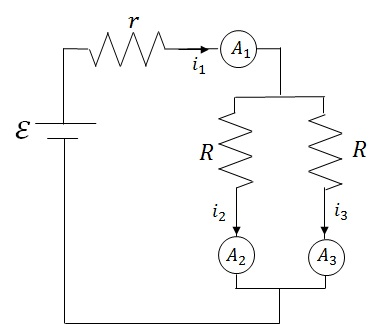
\includegraphics[scale=0.55]{Mallas_sin_carga}
  \caption{Circuito de dos mallas utilizado para la experiencia, los $A_i$ representan los lugares donde se ubicó el multimetro}
  \label{fig:circ_mallas}
\end{figure}

Inicialmente, se utilizaron las leyes de Kirchoff y se resolvió el circuito mediante el método de ramas para obtener el valor de las corrientes $i_1$, $i_2$ e $i_3$ en base a los parámetros. 
 
Luego se ubicó el multimetro en las posiciones $A_1$, $A_2$ y $A_3$ (Ver \textbf{Fig \ref{fig:circ_mallas}}) para medir las corrientes $i_1$, $i_2$ e $i_3$ respectivamente, considerando despreciable la resistencia interna del multímetro.
 
Posteriormente, se buscó calcular el equivalente de Thevenin en forma teórica a través de los parámetros $R$, $r$ del circuito y $\varepsilon$ usando \eqref{Rth} y \eqref{Eth} para obtener la resistencia y la fuente equivalente vista desde las terminales A y B, entre las cuales se conectará una resistencia de carga $R_q$ (ver \textbf{Fig \ref{fig:circ_mallas_carga}}). 

\begin{figure}[h]
  \centering
  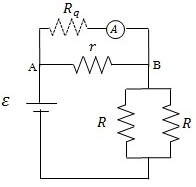
\includegraphics[scale=0.55]{Mallas_con_carga}
  \caption{Circuito de dos mallas con la resistencia de carga acoplada}
  \label{fig:circ_mallas_carga}
\end{figure}



Conectando el multimetro en paralelo en las terminales A y B se midió la diferencia de potencial $\Delta V_{AB}$ y la resistencia $R_{AB}$  entre ambas terminales.

Una vez hecho esto, fue posible conectar una resistencia de carga $R_v$ representada por una resistencia variable por decadas en serie con el multimetro en modo amperimetro. El objetivo fue medir la corriente $I$ para distintos valores de $R_v$ y en base a ambas magnitudes calcular la potencia $P$ disipada por $R_q$ a través de \eqref{Joule} buscando relevar la curva acampanada $P(R_v)$.
%cuyo máximo debería encontrarse en $R_{max} = R_{th}$ $= (83,3\pm0,7)\Omega$ segun (\textbf{POT MAX})



%%%%%%%%%%%%%%%%%%%%%%%%%%%%%%%%%%%%%%%%%%%%%%%%%%%%%%%%%%%%%%%%%%%%%%%%%%%%%%%%%%%%%%%%%%%%%%%%%%%%%%%%%%%%%%%%%%%%%%%%%%%%%%%%
% 4.DISCUSIÓN Y RESULTADOS: todo lo que se obtuvo y explicación. Graficos, tablas.
%%%%%%%%%%%%%%%%%%%%%%%%%%%%%%%%%%%%%%%%%%%%%%%%%%%%%%%%%%%%%%%%%%%%%%%%%%%%%%%%%%%%%%%%%%%%%%%%%%%%%%%%%%%%%%%%%%%%%%%%%%%%%%%%

\section{Resultados}
\label{sec:discusion}

\subsection{Ley de Ohm}

Los resultados de la primer medición con la resistencia $R$ constante pueden verse en la \textbf{Figura \ref{fig:Ohm_lin}}, cuyo ajuste lineal arroja una pendiente $m_1 = (1,979.10^{-3} \pm 5.10^{-6})\Omega^{-1}$ y una ordenada $b_1 = (-0,23\pm 0,03)mA$ muy cercana a cero con un $R-square = 0,99995$, que asegura la bondad del ajuste. Siguiendo \eqref{Ohm}, se esperaría que la pendiente $m_1 = (1,979.10^{-3} \pm 5.10^{-6})\Omega^{-1}$ fuera igual a $\frac{1}{R}$ con $R = (512 \pm 5)\Omega$. Efectivamente, resulta $\frac{1}{m_1} = (505.3 \pm 1,3)\Omega$, el cual se acerca mucho a $R = (512 \pm 5)\Omega$.

\begin{figure}[h]
  \centering
  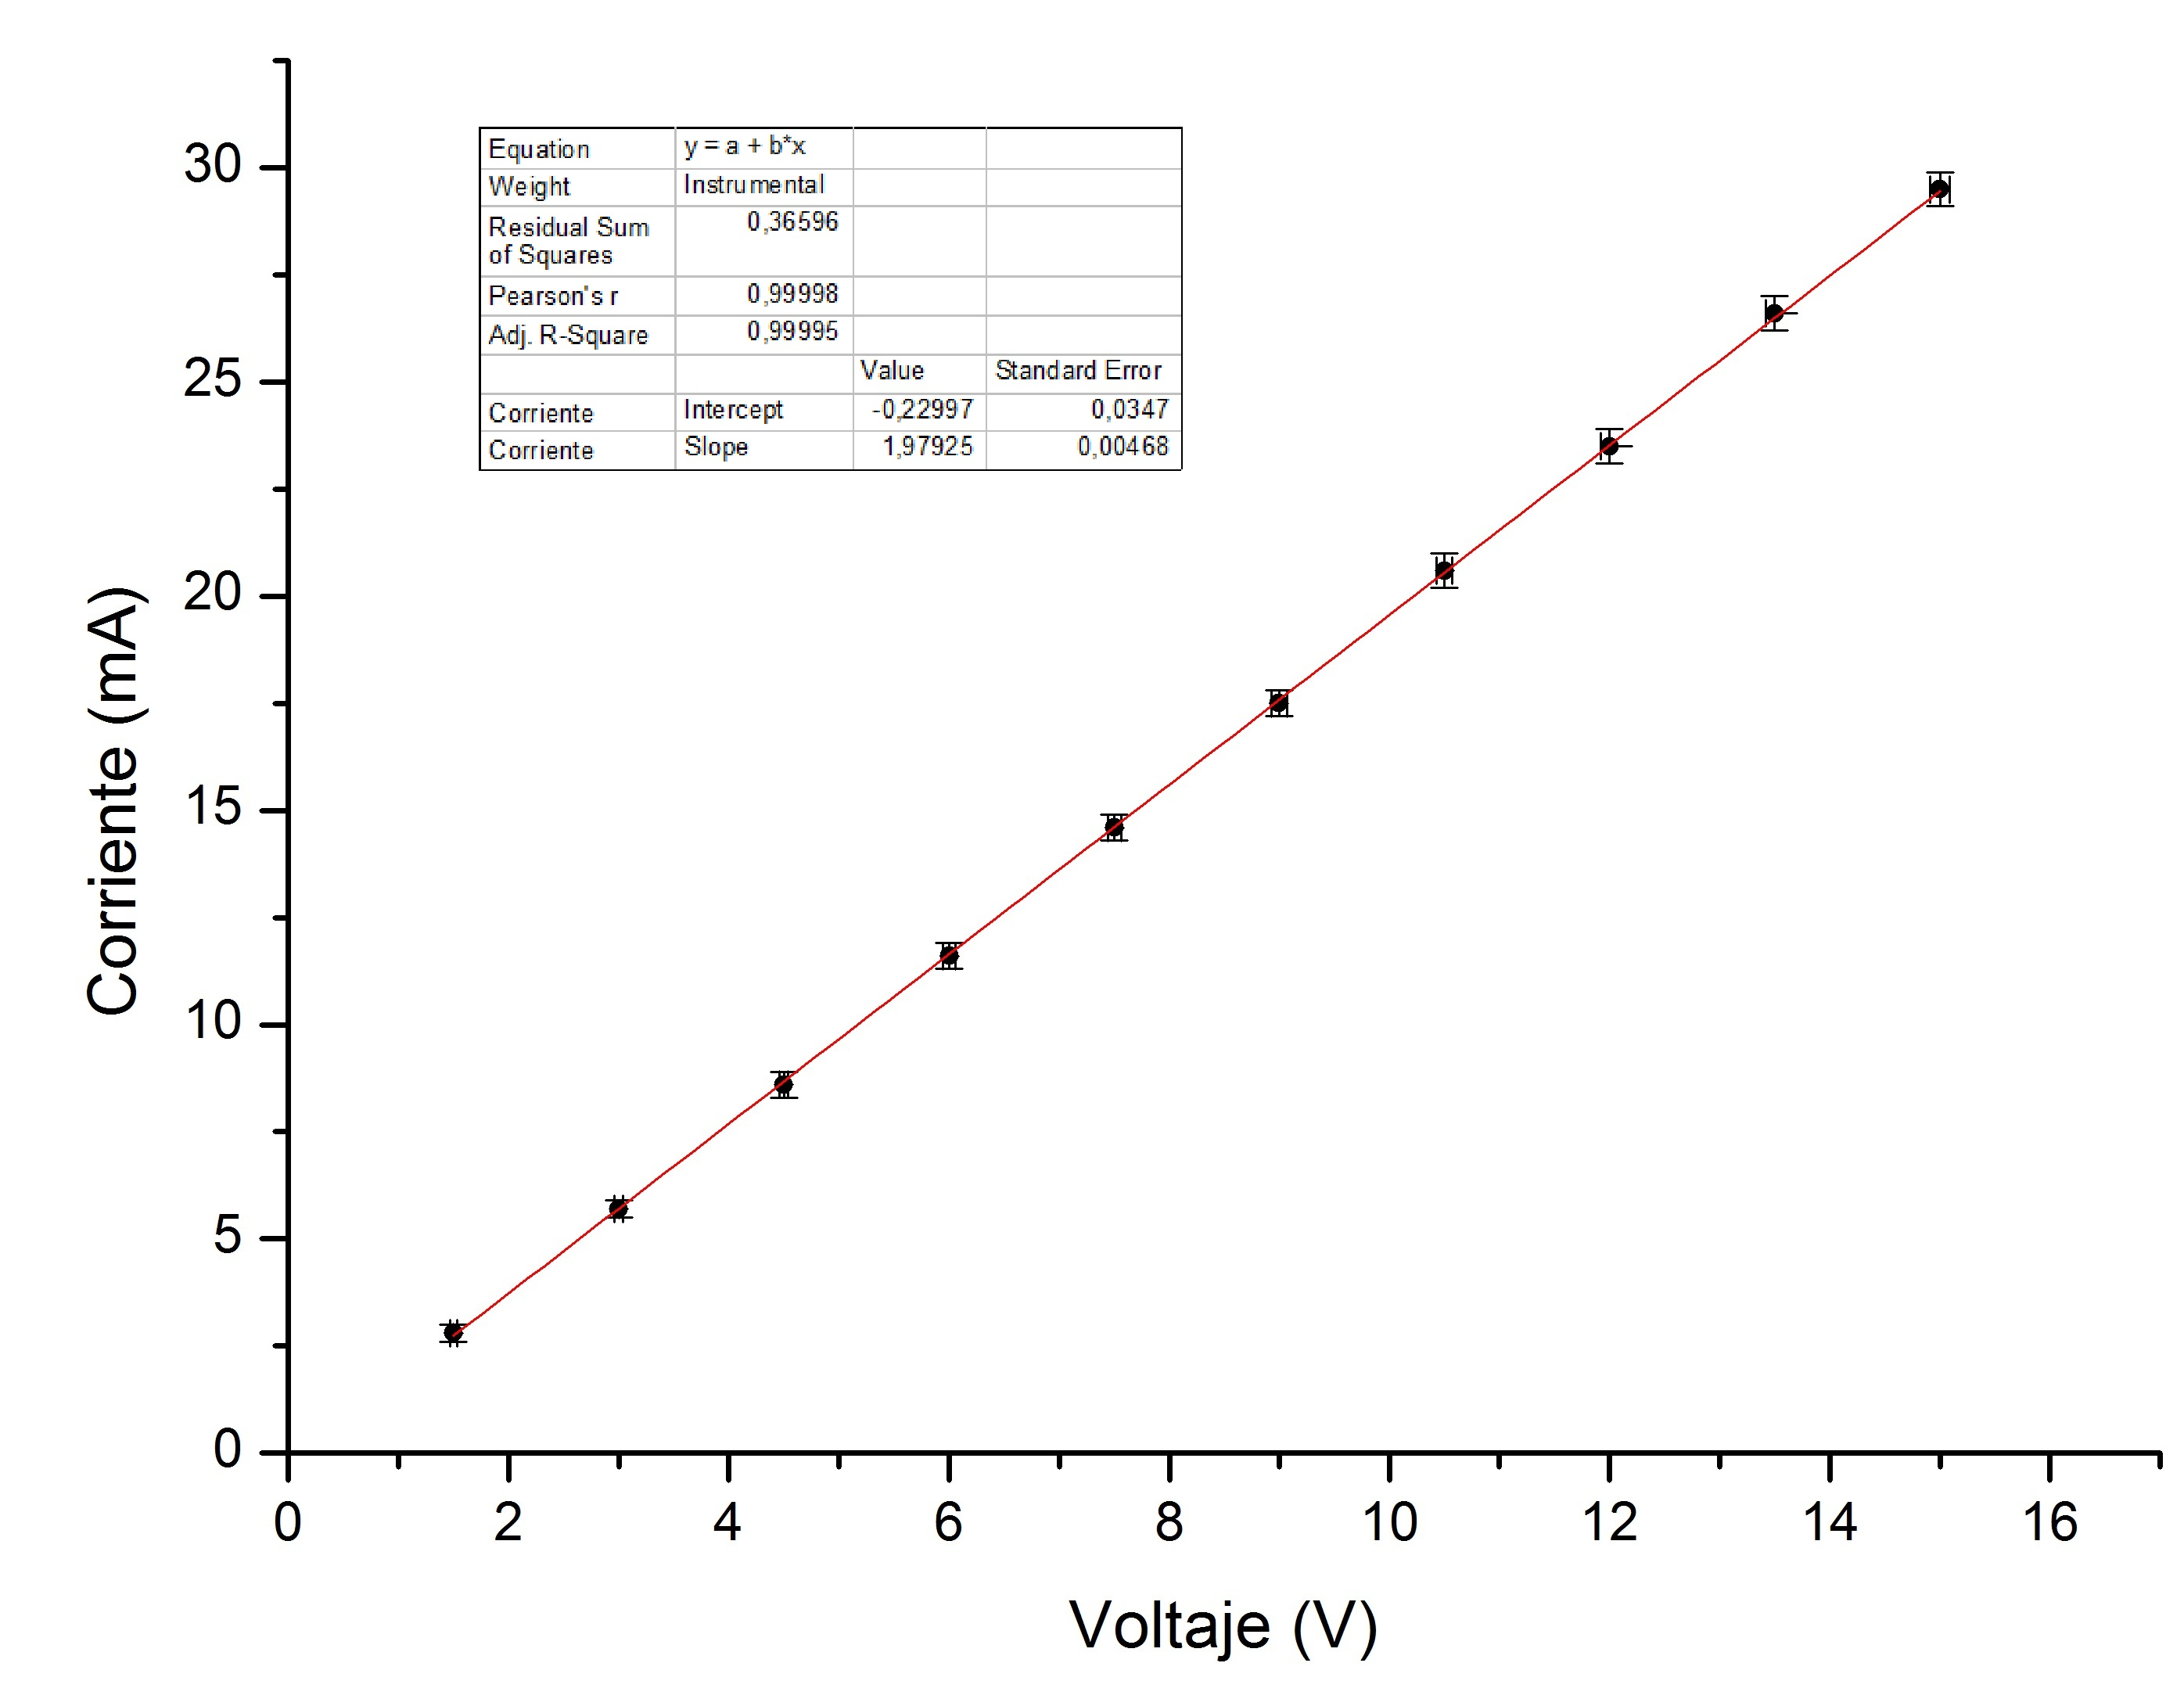
\includegraphics[scale=0.4]{Corriente_vs_Voltaje}
  \caption{Relacion entre Voltaje ($\varepsilon$) y Corriente (I)}
  \label{fig:Ohm_lin}
\end{figure}

Luego, con las mediciones correspondientes a un voltaje constante, se decidio realizar un grafico que relacionara las corrientes medidas con el inverso de las resistencias seleccionadas, de esa forma, si se cumple la ley de Ohm, deberia haber una correspondencia lineal entre esos pares de valores. Como se puede ver en la \textbf{Figura \ref{fig:Ohm_hip}} se confirma lo esperado, ya que una vez realizado un ajuste lineal, nos arroja un $R-square = 0,99958$. Cabe destacar, que para resistencias suficientemente altas, las corrientes resultantes deberian estar por debajo del limite de resolucion de cualquier instrumento de medicion; por lo cual, es consistente que el ajuste nos arroje una interseccion con el eje de ordenadas muy cercano al 0. Efectivamente el valor obtenido es de $b = (-0.001 \pm 0.002)$

%\textbf{OHM HIP}
\begin{figure}[h]
  \centering
  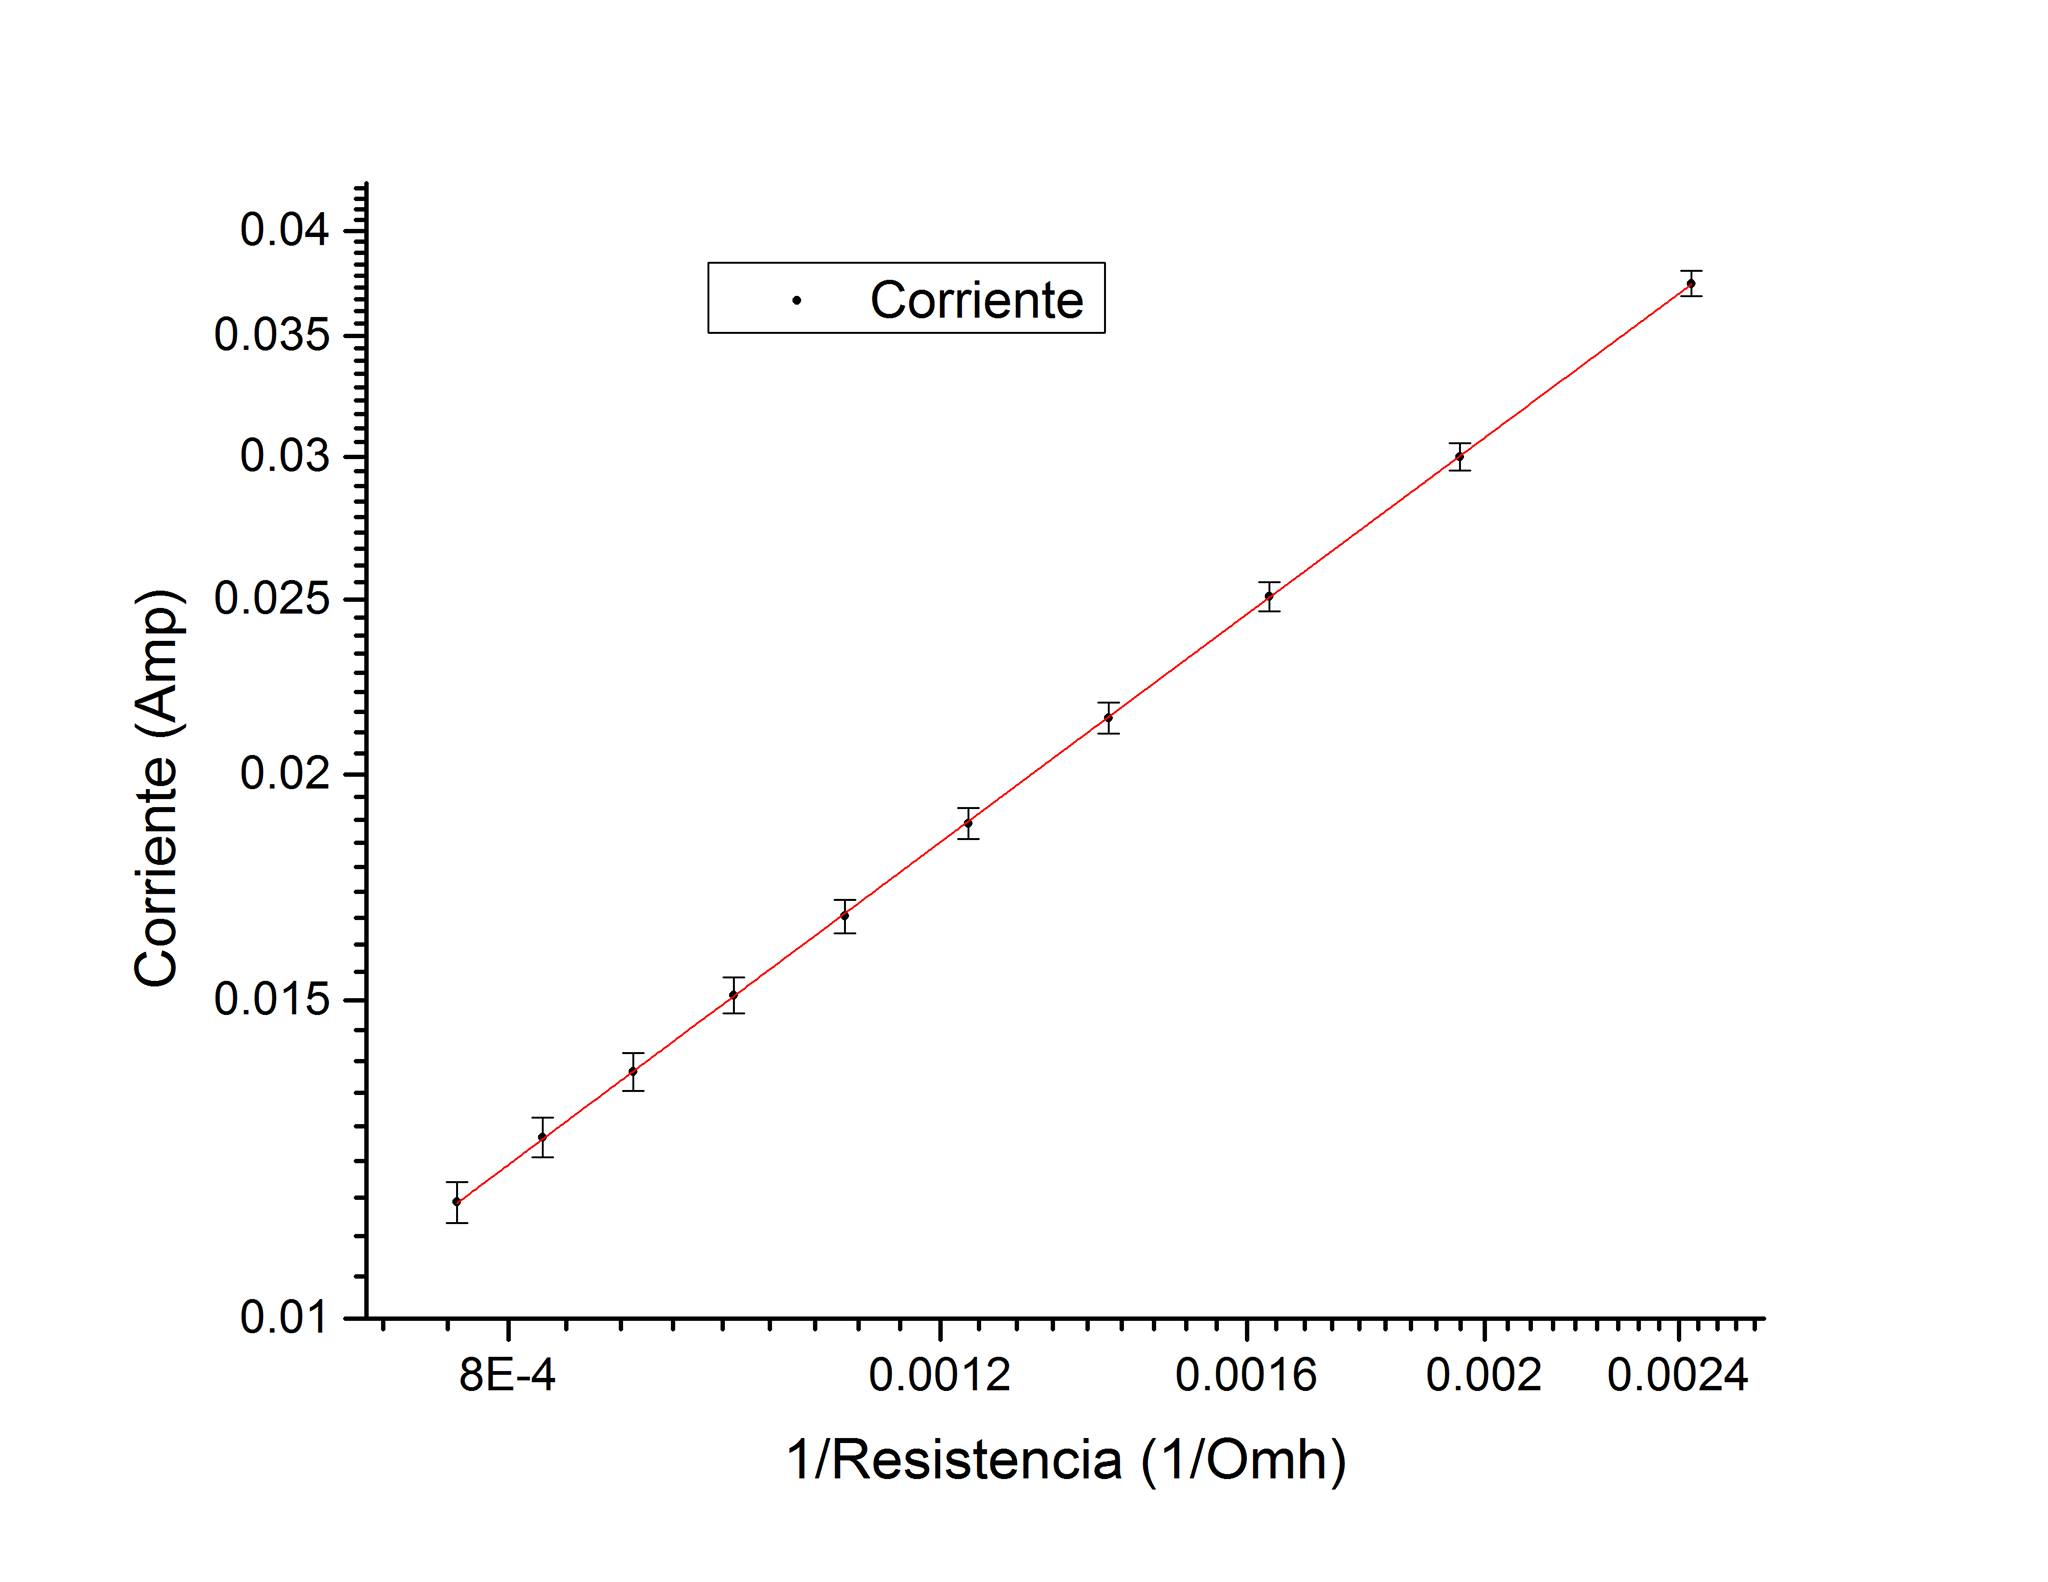
\includegraphics[scale=0.45]{Corriente_vs_InversoResistencia}
  \\[1.0cm]
  \label{fig:Ohm_hip}
  \caption{Relacion entre el inverso de Resistencia (1/R) y Corriente (I)}
\end{figure}

Adicionalmente, segun la ecuacion \eqref{Ohm} se esperaria que la pendiente de esta recta fuera el voltaje de entrada. En este caso resulta ser ligeramente supérior con un valor $m = (16.1\pm0.1) V$

\subsection{Equivalente de Thevenin y Ley de Joule}

 
De las mediciones y calculos hechos de las corrientes $A_1$, $A_2$ y $A_3$ puede verse, en la \textbf{Tabla 1}, que los valores obtenidos con ambos metodos coinciden dentro del error. 

\begin{center}
\begin{tabular}{||c|c|c||}
\hline
& \multicolumn{2}{c||}{\textbf{Valor}} \\ \hline
\textbf{Corriente} & \textbf{Teórico (mA)} & \textbf{Medido (mA)} \\ \hline 
$i_1$ & $8,33\pm0,09$ & $8,3\pm0,3$ \\ \hline 
$i_2$ & $4,17\pm0,05$ & $4,2\pm0,2$ \\ \hline 
$i_3$ & $4,17\pm0,05$ & $4,1\pm0,2$ \\ \hline 
\end{tabular}\\

\textit{Tabla 1: Valores obtenidos de las corrientes mediante cálculo (teórico) y medición directa}
\end{center}

Luego, a través del cálculo del equivalente de Thevenin se obtuvieron los parametros equivalentes $\varepsilon_{th} = (0,83\pm0,08)V$ y $R_{th} = (83,3 \pm 0,7) \Omega$. Cabe aclarar que en este cálculo no intervinieron las corrientes previamente calculadas, si no que se utilizó directamente su dependencia con los parámetros del circuito. Alternativamente, mediante medición directa se obtuvo $\Delta\varepsilon_{AB} = (0,84 \pm 0,06)V$ y $R_{th} = (83,4 \pm 0,6)\Omega$, valores que resultan indistinguibles dentro del error de los anteriormente calculados. 

De los datos obtenidos se obtiene el gráfico de \textbf{Figura \ref{fig:pot_res}} donde se puede observar que el comportamiento de la potencia entregada por el circuito esta dentro de los parametros esperados. Luego, realizando un ajuste, se obtiene una resistencia máxima $R_{max} = (78.5 \pm 0.8)\Omega$ y un voltaje $\varepsilon = (0,74\pm 0,01)V$ ambos muy cercanos a los valores de Thevenin calculados anteriormente.

\begin{figure}[h]
  \centering
  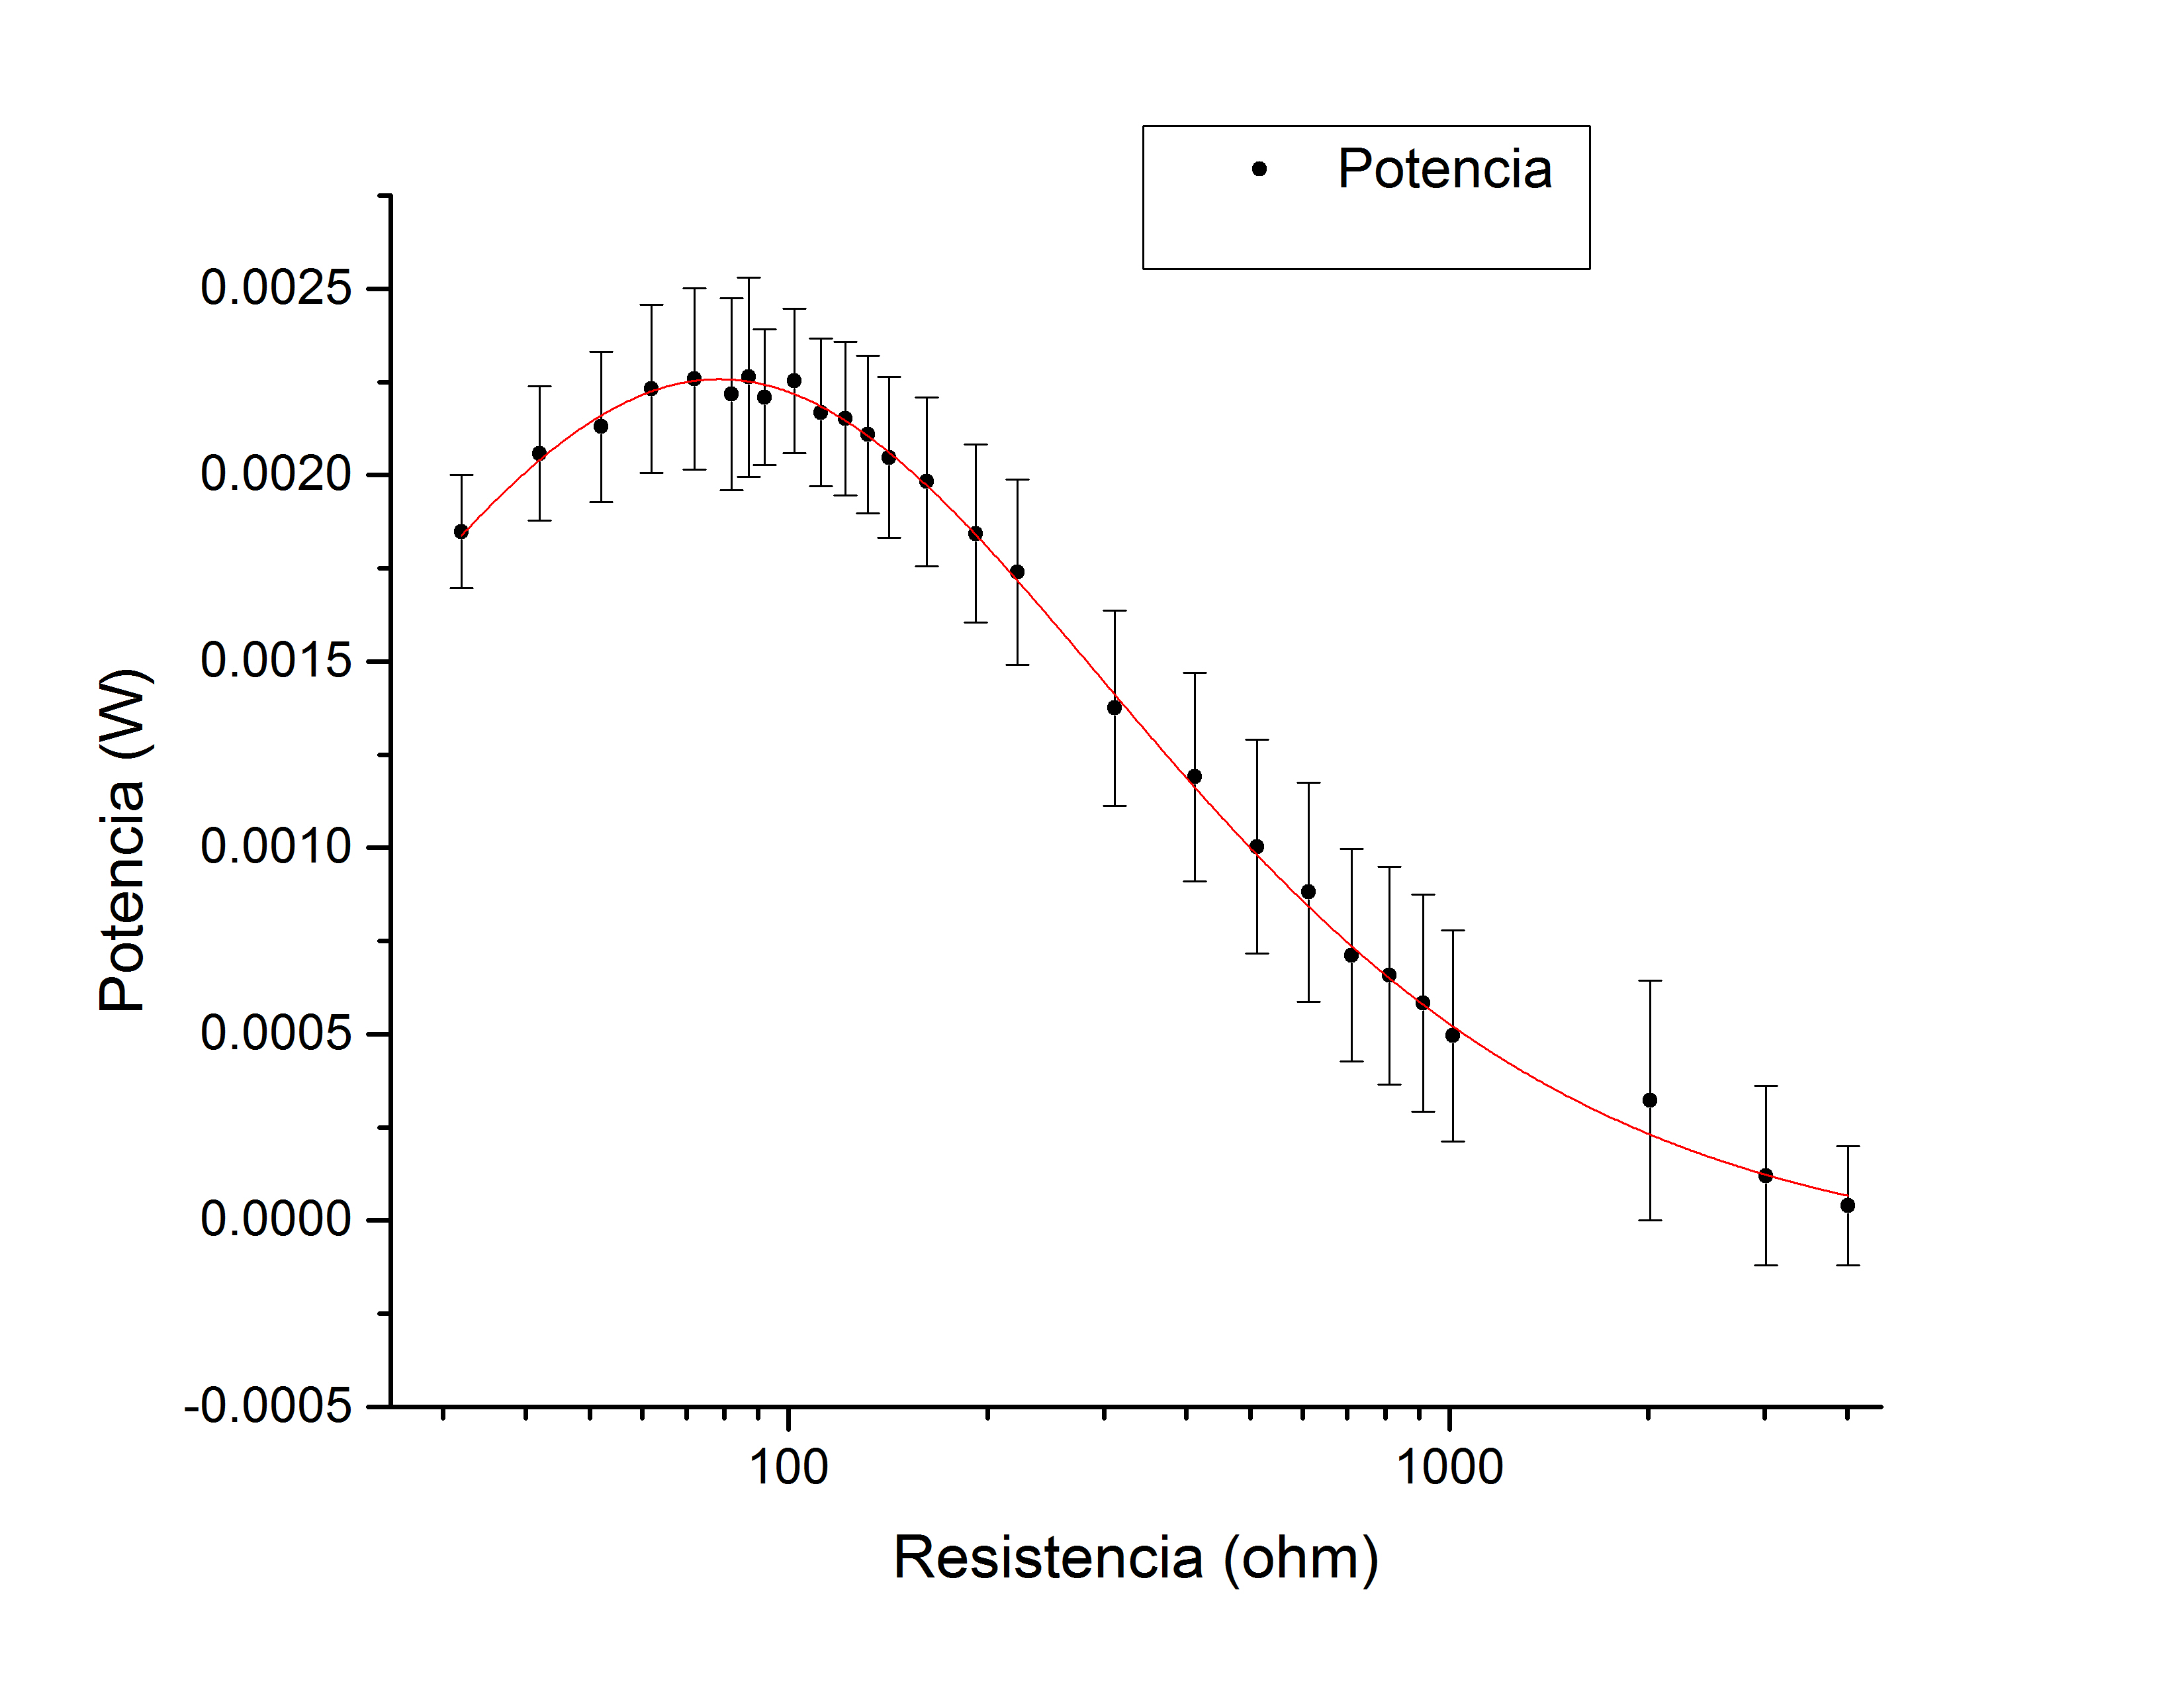
\includegraphics[scale=0.45]{Potencia_vs_Resistencia_2}
  \caption{Relacion entre la potencia disipada y el valor de la resistencia de carga}
  \label{fig:pot_res}
\end{figure}

Finalmente, se calculo la eficacia con la cual se traspasaba la potencia de nuestro circuito sobre la carga. En el grafico de la \textbf{Figura \ref{fig:efi_res}} se ve que hay una tendencia creciente pero que en los ultimos puntos se empieza a dispersar. Esto puede deberse a queal trabajar con resistencias tan altas, las corrientes medidas quedan muy cerca del umbral de resolucion del multimetro, por lo cual ya las fluctuaciones propias del instrumento provocan incertezas muy altas. 

\begin{figure}[h]
  \centering
  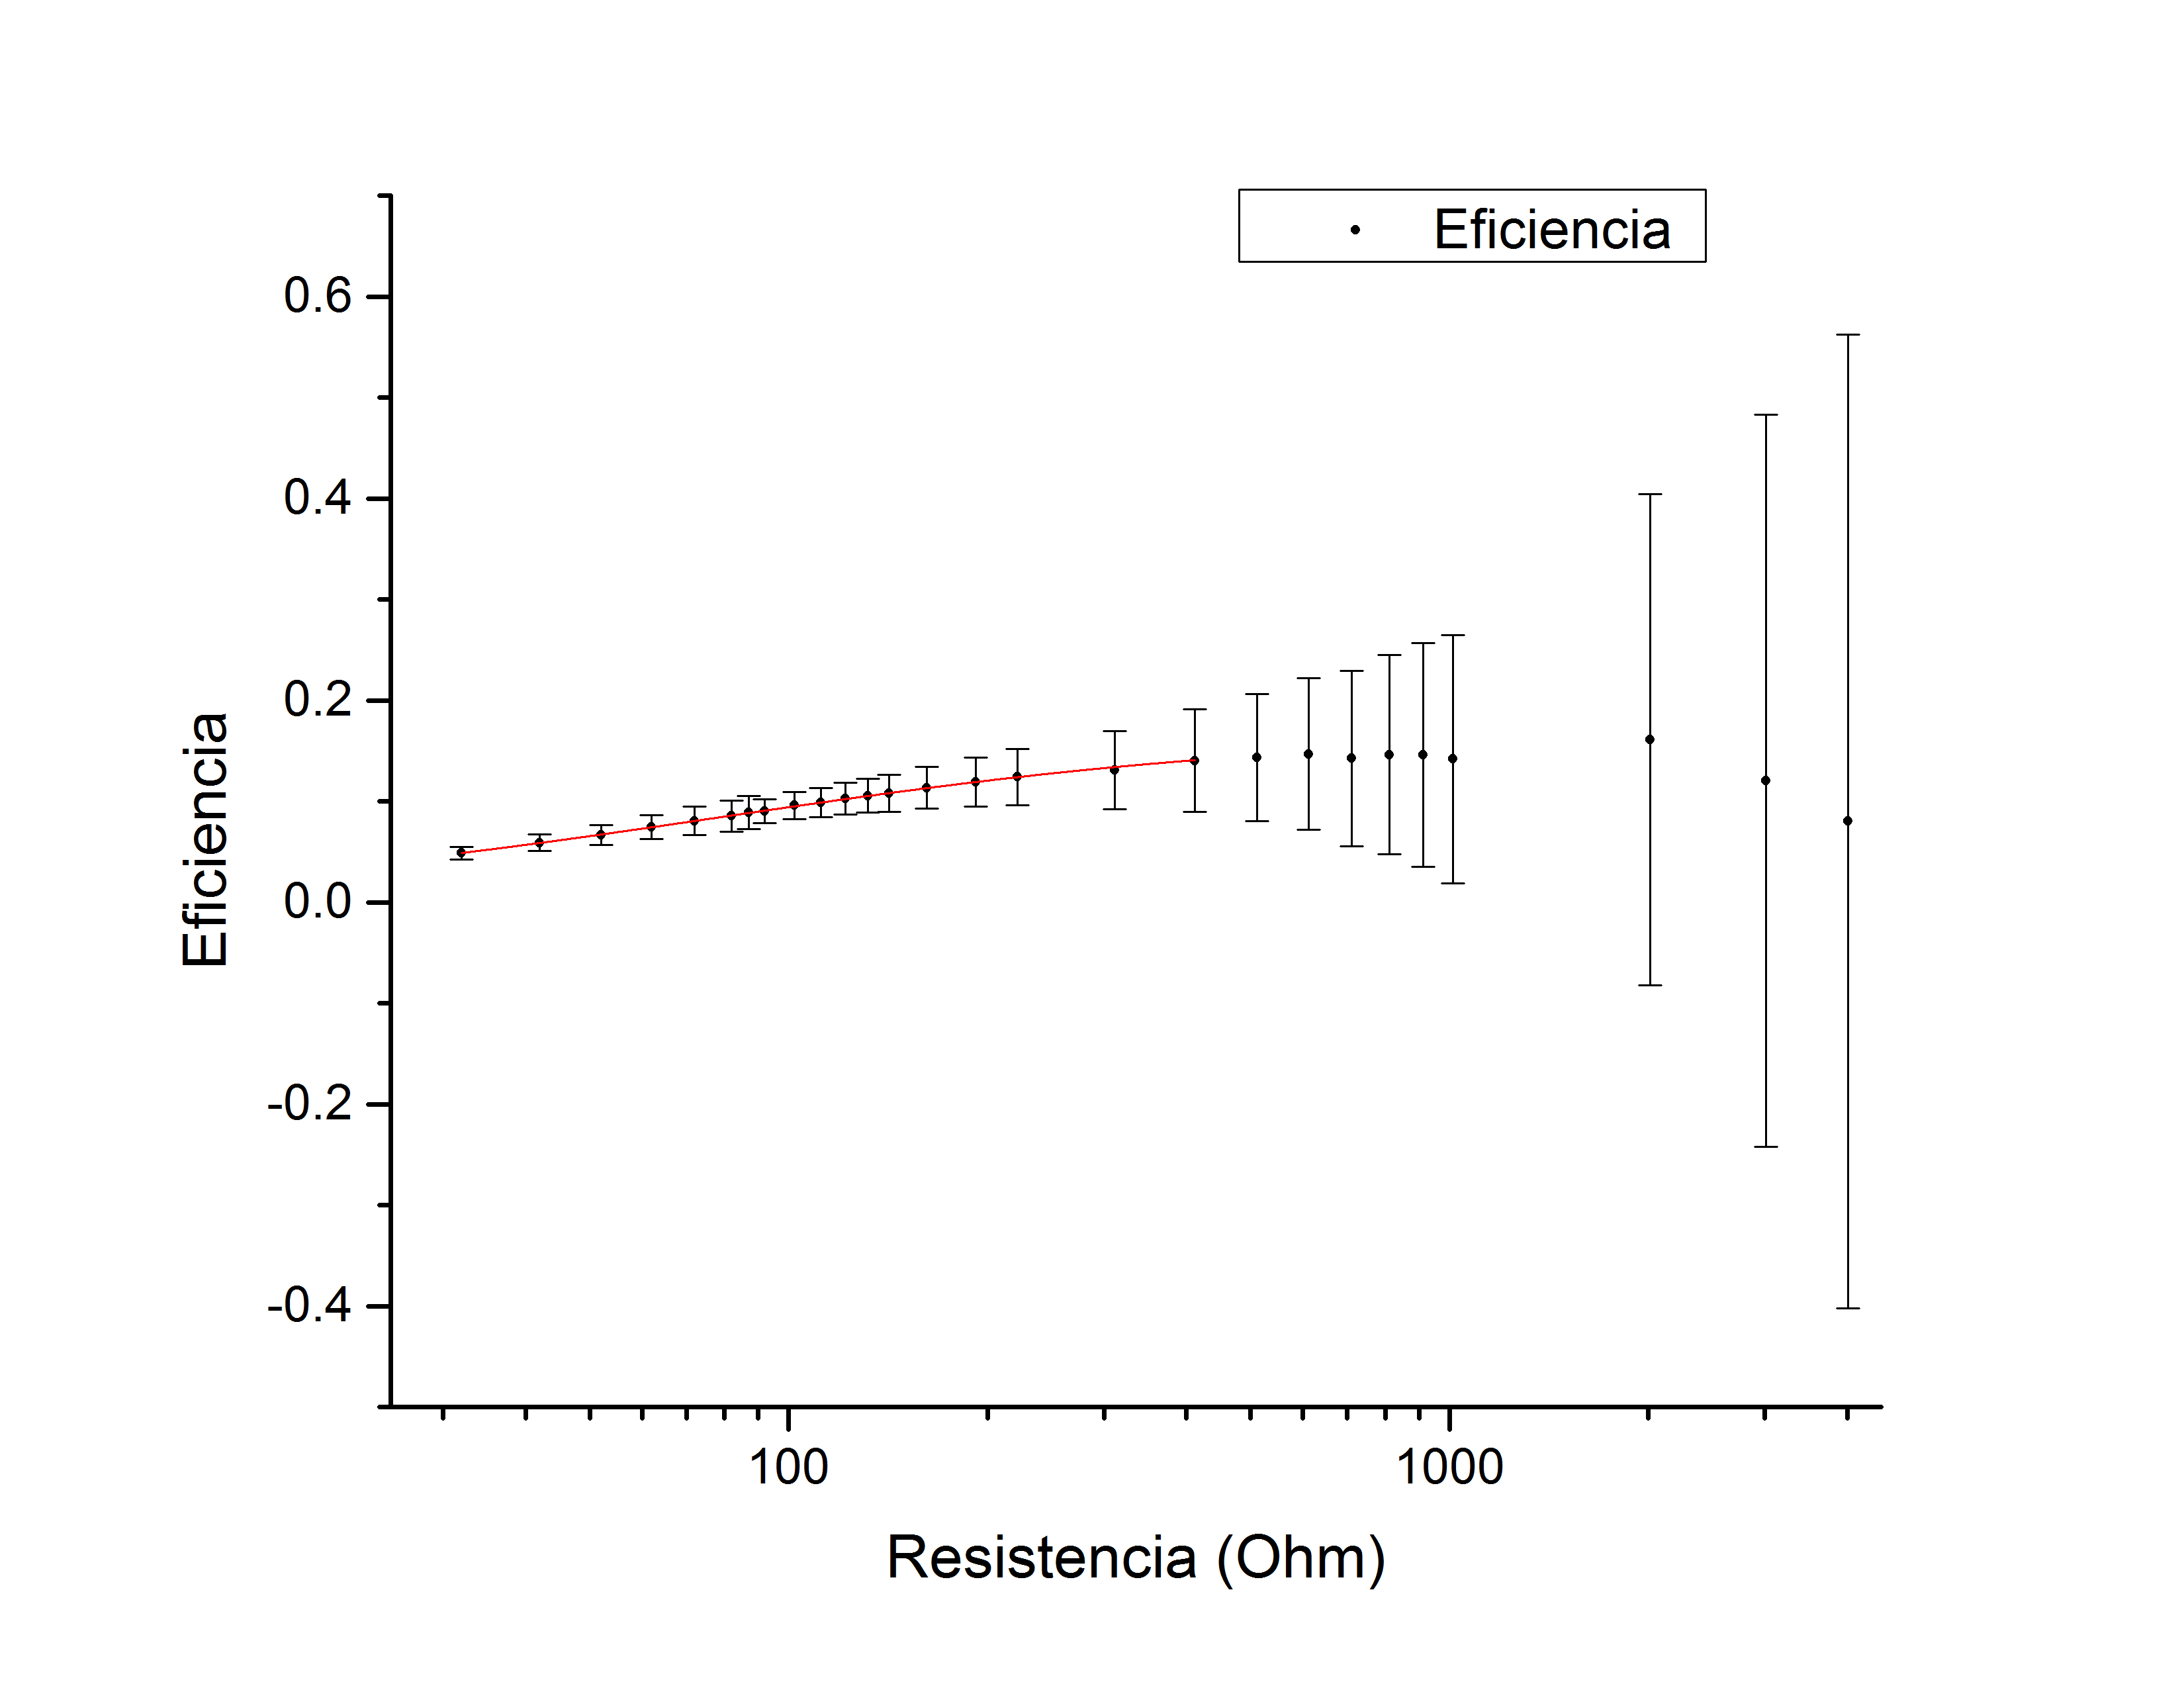
\includegraphics[scale=0.45]{Eficiencia_vs_Resistencia}
  \caption{Relación entre la eficacia de la entrega de potencia y el valor de la resistencia de carga}
  \label{fig:efi_res}
\end{figure}

Desestimando los puntos en cuyos calculos contenian corrientes con incertezas comparables con sus mediciones, el ajuste realizado utilizando \eqref{efi} arroja como uno de sus parametros, la resistencia equivalente del circuito $R_{max} = (77.8 \pm 0.8)\Omega$ que es consistente con los resultados y mediciones anteriores.



%%%%%%%%%%%%%%%%%%%%%%%%%%%%%%%%%%%%%%%%%%%%%%%%%%%%%%%%%%%%%%%%%%%%%%%%%%%%%%%%%%%%%%%%%%%%%%%%%%%%%%%%%%%%%%%%%%%%%%%%%%%%%%%%
%	CONCLUSIONES
%%%%%%%%%%%%%%%%%%%%%%%%%%%%%%%%%%%%%%%%%%%%%%%%%%%%%%%%%%%%%%%%%%%%%%%%%%%%%%%%%%%%%%%%%%%%%%%%%%%%%%%%%%%%%%%%%%%%%%%%%%%%%%%%

\section{Conclusiones}
\label{sec:conclusiones}




%%%%%%%%%%%%%%%%%%%%%%%%%%%%%%%%%%%%%%%%%%%%%%%%%%%%%%%%%%%%%%%%%%%%%%%%%%%%%%%%%%%%%%%%%%%%%%%%%%%%%%%%%%%%%%%%%%%%%%%%%%%%%%%%%
%	APÉNDICE: esas cosas extras que simplemente no tuvieron lo suficiente como para ganarse una sección propia.
%%%%%%%%%%%%%%%%%%%%%%%%%%%%%%%%%%%%%%%%%%%%%%%%%%%%%%%%%%%%%%%%%%%%%%%%%%%%%%%%%%%%%%%%%%%%%%%%%%%%%%%%%%%%%%%%%%%%%%%%%%%%%%%%%



%%%%%%%%%%%%%%%%%%%%%%%%%%%%%%%%%%%%%%%%%%%%%%%%%%%%%%%%%%%%%%%%%%%%%%%%%%%%%%%%%%%%%%%%%%%%%%%%%%%%%%%%%%%%%%%%%%%%%%%%%%%%%%%%%
%	REFERENCIAS: libros, libros, libros.
%%%%%%%%%%%%%%%%%%%%%%%%%%%%%%%%%%%%%%%%%%%%%%%%%%%%%%%%%%%%%%%%%%%%%%%%%%%%%%%%%%%%%%%%%%%%%%%%%%%%%%%%%%%%%%%%%%%%%%%%%%%%%%%%%

%Ejemplo:
\begin{thebibliography}{1}
 \bibitem{Berkeley} Frank S. Crawford, \textit{Berkeley physics course 3: Ondas}, 1994, Editorial Reverte S.A.
\end{thebibliography}
%Para citar: blablabla \cite{Baird}
 
\end{document}





